Uno de los desafíos más grandes en este proyecto era migrar el código de MODNET a python. Para comenzar, se le solicitó al laboratorio TIMA el código actual en C\# para comenzar su estudio.

Fue una sorpresa encontrarnos que el código estaba prácticamente abandonado desde el 2013 y no había una última versión clara, se encontró una versión en internet que se obtuvo desde la tesis en PDF de Wassim, y el resto del código original de lo provisto por el laboratorio que se encontraba en un disco externo en Francia.

Una vez con el código en mano, se decidió subir una primera release a GitHub del código original en C\#, para así preserver tanto el legado del doctor Wassim, como así también para facilitar el trabajo a desarrollar en la migración.

Una de las primeros bloqueos que se encontraron fue que el código de MODNET debía ser recompilado para cada DUT que se quisiera someter bajo prueba. Es decir, que para poder siquiera implementar un cambio mínimo en un diseño RTL, era necesario contar con la suite completa de Visual Studio 2012. Además, la ubicación de la NetList debía ser configurada en tiempo de compilación como se observa en la figura ~\ref{modnet_gui_1}, complicando aún más el uso de la herramienta.

\begin{figure}[H]
	\centering
	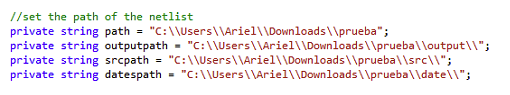
\includegraphics[width=1 \textwidth, frame]{img/modnet_gui_1.png}
	\caption{ Código original que solicitaba definir la ubicación de la NetList en tiempo de compilación}
	\label{modnet_gui_1}
\end{figure}

Por otra parte, el código original era muy complicado de interpretar y seguir. Se podían observar mucha cantidad de modificaciones de string sin ninguna explicación, como la inclusión de diversos caracteres que moficicaban el comportamiento del DUT sin siquiera un comentario de porque se realizaba. Como ejemplo, en la figura ~\ref{modnet_gui_5} se muestra el código que inserta una entrada de inyección de fallo si: 

\begin{enumerate}
    \item La línea contiene 2 caracteres especiales, un espacio en blanco y un paréntesis abierto,
    \item si la lógica es de tipo secuencial,
    \item si el tipo de error es SEU.
\end{enumerate}

\begin{figure}[H]
	\centering
	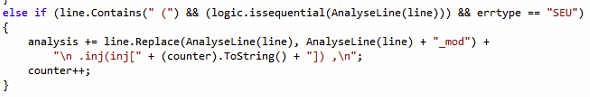
\includegraphics[width=\linewidth, frame ]{img/modnet_gui_5.png}
	\caption{ Insersión de un lugar a inyección de fallo por MODNET original}
	\label{modnet_gui_5}
\end{figure}

Esto no es solo confunso, sino que además imposibilita por completo a la extensión del proyecto. ¿Qué significa `` ('' ? ¿Es específico a la NetList de Synplify?. Estas son algunas de las preguntas que surgieron durante el desarrollo que se intentaron solucionar a partir de la implementación de clases en python, abstrayendo así al programador dentro de la lógica de inyección de fallas sobre como está elaborada la NetList, y asi acelerando el proceso de desarrollo.

Por otra parte, la implementación de MODNET requería de la interacción con una GUI, que se ve en la figura \ref{modnet_gui_4}. Es decir, que si se solucionaban algunos de los problemas anteriormente nombrados, aún se estaba atado a tener que lidiar con una interfaz gráfica que no permitiría la automatización del sistema.

\begin{figure}[H]
	\centering
	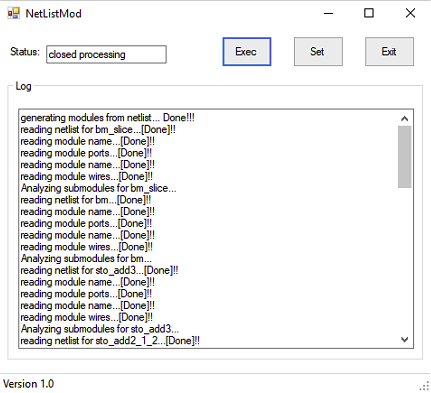
\includegraphics[width=0.6 \textwidth, frame]{img/modnet_gui_4.png}
	\caption{Ejecución de un proceso de inyección de lugares de falla en MODNET v1.}
	\label{modnet_gui_4}
\end{figure}

En la figura \ref{modnet_python_1} podemos observar la misma sección de código luego de ser traducida a python. En la misma se puede observar como `` ('' se convierte en un atributo de la clase \textit{ModuleCst} llamado \textit{COMPONENT\_START}, de esta manera queda claro que se comienza a iterar en busca de puntos sensibles de inyección a partir del comienzo de la declaración de un componente (por ejmplo, una LUT), haciendo el código más legible y fácil de seguir. Por otro lado, esto facilita la extensión de MODNET v2 hacia otro tipo de NetLists, ya que basta con definir un tipo de \textit{COMPONENT\_START} para cada netlist (como puede ser, una para Synplify y otro para Yosis), haciendo que la lógica que busca puntos sensibles no deba cambiar, simplemente se comportará de manera distinta dependiendo del tipo de NetList que se esté procesando.

\begin{figure}[H]
	\centering
	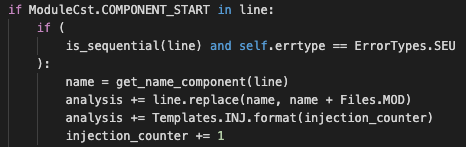
\includegraphics[width=0.8 \textwidth]{img/modnet_python_1.png}
	\caption{ Insersión de un lugar a inyección de fallo por MODNET v2}
	\label{modnet_python_1}
\end{figure}

Se puede observar además como el lugar de inyección ahora parte de un \textit{template} de la clae \textit{Templates}, en donde se define que una inyección para Synplify tiene el formato \path{inj[]}, pudiendo así extender para otras NetLists como debería representarse dentro de un componente el inicio de un punto sensible o lugar de inyección. Estos son solo algunas de las mejoras que se implmentarond de cara a la migración a Python 3. El seguimiento y esquema de release del proyecto se encuentran dentro del repositorio de GitHub donde se puede apreciar todas las etapas por las cuales se sometió a la implementación original.